\section{Methodologies}
\label{methods}
\subsection{Game simulation}

To simulate the entirety of a game, we utilized a combined ASP and Python framework, which is summarized in a later subsection. In regards to ASP, we created an encoding, namely \texttt{background.lp}, representing the dynamics of the game to perform a single time step. This encoding depends on a set of facts defining the current state of the game. For the initial state, such facts are saved in a file and for the following states, they are computed throughout the simulation. Initial states are saved in files \texttt{*initial.lp}, where * implies a prefix. Both sets of encodings are written using the GDL formalisms, such that the same variable and atom naming conventions can be used across all games. For the game of Nim illustrated in Figure 4, the background program and initial state can be found in Figure 5 and Figure 6, respectively. 

\lstset
{ %Formatting for code in the appendix
    language=Prolog,
    basicstyle=\footnotesize,
    numbers=left,
    stepnumber=1,
    showstringspaces=false,
    tabsize=1,
    breaklines=true,
    breakatwhitespace=false,
    frame=single,
    xleftmargin=2em
}

\begin{center}
    \begin{lstlisting}[] 
#const max_removable = 6. 
#const max_sticks = 7. 
#const num_piles = 4.

% Roles
role(a). role(b).

% Base (All possible values inside 'true')
base(has(P,M)):- P=1..num_piles,M=0..max_sticks.
base(control(X)) :- role(X).

% Input (All possible actions)
input(X,remove(P,N)) :- P=1..num_piles, 
                        N=1..max_removable,
                        role(X).

% Legal actions
legal(X,remove(P,N)) :- true(has(P,M)), 
                        P = #min{L:true(has(L,M))},
                        N=1..max_removable, N<=M, 
                        true(control(X)), 
                        not terminal.

% Action selection
0 {does(X,A)} 1 :- legal(X,A), not terminal.
:- does(X,Y), does(X,Z), Y < Z.
:- not does(X,_), true(control(X)), not terminal.

% State transition
next(control(b)) :- true(control(a)), not terminal.
next(control(a)) :- true(control(b)), not terminal.
next(has(P,N-M)) :- does(_,remove(P,M)), 
                    true(has(P,N)), not terminal.
next(has(P,N)) :- not does(_,remove(P,_)), 
                  true(has(P,N)), not terminal.

% Goals
goal(X,-1) :- #sum{N,M:true(has(M,N))}=0, true(control(X)).
goal(X,-1*G):- goal(Y,G), role(X), X!=Y.

% Terminal state
terminal :- goal(_,_).
    \end{lstlisting}
    \captionof{figure}{\texttt{background.lp} encoding for dynamics of the game of Nim}
\end{center}

\begin{center}
    \begin{lstlisting}[] 
true(has(1,3)).
true(has(2,1)).
true(has(3,0)).
true(has(4,0)).
true(control(a)).
    \end{lstlisting}
    \captionof{figure}{ASP encoding the initial state of Figure 4}
\end{center}

Throughout the game simulation, each node $T(i,j,p,d)$ of the tree can expanded with the following actions. Using the background program $P$ and the set of facts representing the state $T(i,j,p,d)[s]$, we call \textit{clingo} in search for the next possible states. This call will obtain one answer set per legal action. For each answer set, we proceed to create a new children node $T(i,j',p',d+1)$ were its state $T(i,j',p',d+1)[s]$ is constructed by replacing $\texttt{next/1}$ with predicate $\texttt{true/1}$. To exemplify such process, show the output when we call \textit{clingo} with the encodings from Figure 5 and Figure 6. This call will return 4 answer sets corresponding to the first level of the tree in Figure 4.

\begin{figure}[H]
\centering
\begin{varwidth}{\linewidth}
\begin{verbatim}
Answer: 1
next(has(3,0)) next(has(4,0)) next(control(b))
does(a,remove(2,1)) next(has(1,3)) next(has(2,0))

Answer: 2
next(has(3,0)) next(has(4,0)) next(control(b)) 
does(a,remove(1,2)) next(has(2,1)) next(has(1,1))

Answer: 3
next(has(3,0)) next(has(4,0)) next(control(b)) 
does(a,remove(1,3)) next(has(2,1)) next(has(1,0))

Answer: 4
next(has(3,0)) next(has(4,0)) next(control(b)) 
does(a,remove(1,1) next(has(2,1)) next(has(1,2))
\end{verbatim}
\end{varwidth}
\end{figure}

Using the Python Application Programming Interface (API) for \textit{clingo}, we can then extrapolate this process to simulate multiple time steps in the game and construct the game tree. Further, when given a strategy in the form of weak constraints, such encoding can be included, enforcing an order over the answer sets. Such ordering will allow the player you select the best action (answer set) according to the optimization defined by the weak constraints.


\subsection{Learning Approaches}

\subsubsection{Minimax Algorithm}

The minimax algorithm is a recursive tree-search algorithm which has its origins in combinatorial game theory for choosing the next best move of a two-person zero-sum game. The intuition behind this algorithm lays in the fact that every movement made by player $a$ will aim to maximize the reward of $a$, while player $b$ will try to minimize this same reward. This algorithm will first construct the complete game tree $T$ of depth $D$ for alternately-playing players $p$ and $p'$. All the terminal nodes of the tree will be annotated with reward values $v$ extracted from predicate $\texttt{goal/1}$. Then, it will proceed to compute the minimax score $M$ of any node on the tree starting on the leaves by utilizing the following piecewise function:

\begin{equation}
M(j,p,d-1) = 
\begin{cases} 
\underset{k}{\max} ~ T(j,k,p',d)[v], & p = a\\[10pt]
\underset{k}{\min} ~ T(j,k,p',d)[v], & p = b\\[10pt]
\end{cases}
\end{equation}

\justify
where:
\begin{flalign*}
~~~ &d = \text{depth of node on the decision tree: } d \in [0,D], ~ d \in \mathbb{N}_0& \\
~~~ &j = \text{$j$'th parent node on depth $d-1$ where $M$ is to be evaluated: } j \in \mathbb{N}_0& \\
~~~ &k = \text{$k$'th child node of parent node $j$ on depth $d$ where $v$ is defined: } k \in \mathbb{N}_0& \\
%~~~ &M(i,p,D) = T(i,p,D)[v]\text{: minimax values at leaves are equal to reward values}& \\
~~~ &p, p' = \text{unique player playing on specified depth:} ~ p,p' \in {\cal P} = \left\{a,b\right\},~ p' = {\cal P} \setminus p &\\
~~~ &\textbf{Note: } \text{We assume the positive reward player $a$ maximizes $M$ while the}& \\
~~~ &\text{negative reward player $b$ minimizes $M$} &
\end{flalign*}

\justify
Given the piecewise function $M$ defined above, we present below the pseudocode used for the minimax algorithm in our project. The time complexity of this algorithm is $O(b^D)$, while the space complexity is $O(bD)$; where $b$ is the average branching factor and $D$ is the maximum depth of the game tree \citep{russell2016artificial}.

\begin{algorithm}
  \caption{Minimax}
  \begin{algorithmic}[1]
  \Require{Game tree $T$ of depth $D$ with reward values $v$ at terminal nodes}
  \Ensure{Game tree $T'$ with minimax values at all nodes}
  \Statex
    \Function{Minimax}{$T$}
      \State $T' \gets T$ \Comment{Make local copy of $T$ as $T'$}
      \For{$d \gets D-1$ to $0$} \Comment{Loop upwards from bottom of $T'$}
      \ForEach{node $T(i,j,p,d)$} \Comment{Loop each node at depth $d$}
        \State $T'(i,j,p,d)[v] \gets M(j,p,d)$ \Comment{Update $T'$ with $M$}
      \EndFor
      \EndFor
      \State \textbf{return} $T'$ \Comment{Return updated game tree $T'$}
    \EndFunction
  \end{algorithmic}
\end{algorithm}

\begin{figure}[H]
  \centering
  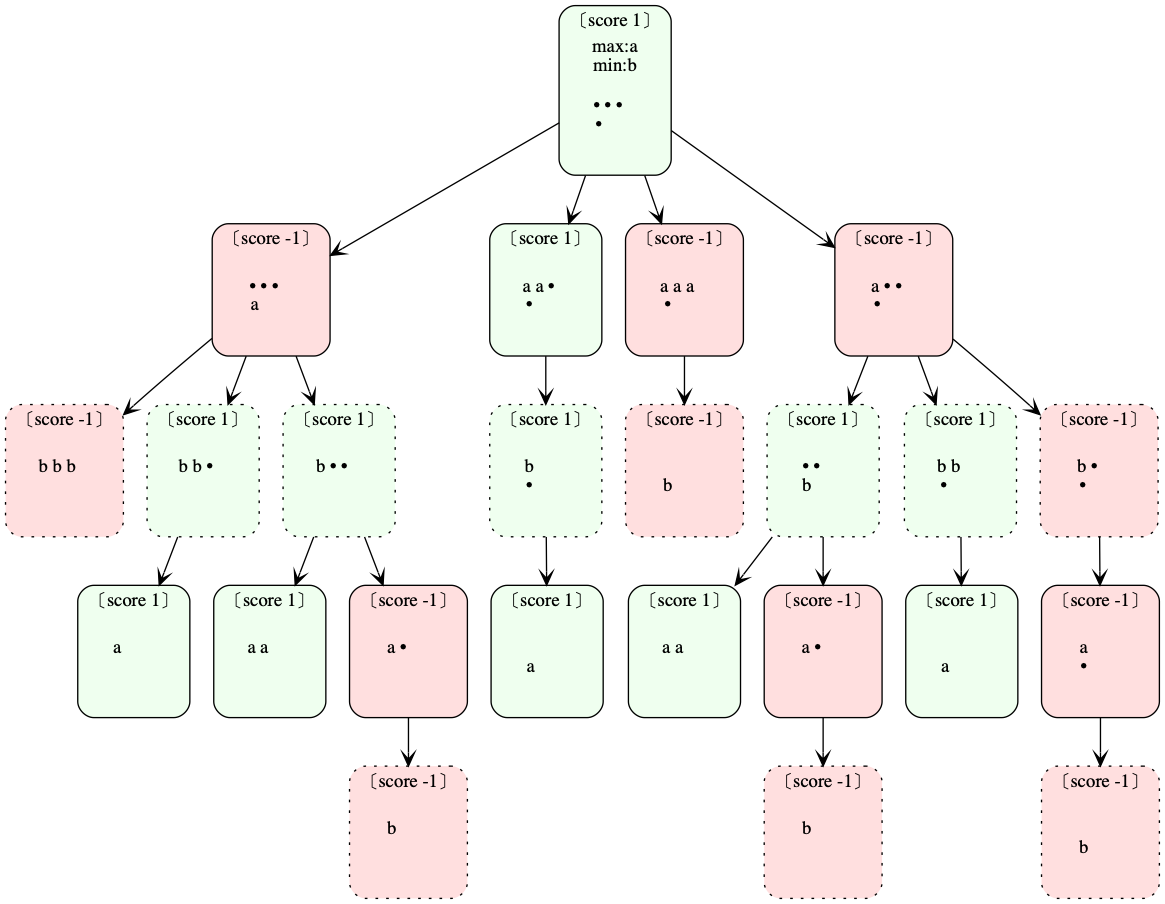
\includegraphics[width=0.9\linewidth]{tree-minmax.png}
  \caption{Tree resulting from applying the Mimimax algorithm to the complete tree in Figure 4. Green nodes have a positive score, implying a winning strategy for player $a$, while red nodes represent an position where player $b$ will win.}
\end{figure}

In the example given on Figure 7, all nodes are scored using the minimax function $M$, defined in formula 1. Since the score of the root node is $1$, player $a$ can assure a winning outcome by following the path down the tree choosing the nodes that have this score, such nodes are marked in green. We can notice this path is the same one as the one defined on Figure 1.

\subsubsection{Pruned Minimax Algorithm}

The Minimax algorithm has many variants that aim to make it more efficient by decreasing the number of nodes that are evaluated. One of the best-known algorithms, called Alpha–beta pruning \citep{knuth1975analysis}, stops evaluating a move when at least one possibility has been found that proves the move to be worse than a previously examined move. Our proposed Pruned Minimax algorithm is based on this idea while including the optimization statements existent in \textit{clingo}. The construction is performed similarly to the Depth-first search (DFS) algorithm for traversing or searching tree. 

\vspace{10px}
\textbf{Explicit time encoding}\\

In GDL we use predicate \texttt{true(F)} to indicate that \texttt{F} holds in the current state and \texttt{next(F)} when it holds in the next state. This syntax can be translated to a single predicate \texttt{holds(F,T)} where the time step in which \texttt{F} holds is specified with \texttt{T}. This notation is used for planning problems and it is based on event calculus \cite{shanahan1999event}. 
With the new encoding, each stable model will represent a full match containing the actions performed in each time step.
This representation makes use of all the advantages provided by \textit{clingo} for planning problems such as incremental solving. In order to translate our current encoding to this new format we need to perform the following steps:
\begin{enumerate}
\item Replace \texttt{true(F)} by \texttt{holds(F,T)}
\item Replace \texttt{next(F)} by \texttt{holds(F,T+1)}
\item Replace \texttt{p(F1..Fn)} by \texttt{p(F1..Fn,T)} where $p\in \{ legal,does,goal,terminal\}$
\item In every rule where a replacement was made, add the time in in the body with predicate \texttt{time(T)}.
\item Add a new fact with all possible time steps \texttt{time(0..N)} using a predefined horizon $N$.
\end{enumerate}


\vspace{10px}
\textbf{Optimization}\\

The system \textit{clingo} comes with a set of optimization statements that enforce an order in the answer sets. With the optimization statement \\ 
\texttt{\#maximize\{N,T:goal(a,N,T)\}} 
we can find the stable model which maximizes the reward $N$ given to player $a$ defined in the predicate \texttt{goal(a,N,T)}, 
were $T$ is the time step in which the goal was reached. By adding this to the explicit time encoding of a game, we will find the match that maximizes the reward for $a$. 
However, this optimization assumes that player $b$ will make the moves that generate the best outcome for his opponent. 
We will call this match $\mathcal{M}_a$ an optimized match for $a$. 
To select actions for player $b$ working on his own benefit, we would need to minimize the reward of $a$ in the time steps where player $b$ has control. 
Minimizing the reward of $a$ can be achieved with the optimization statement 
\texttt{\#minimize\{N,T:goal(a,N,T)\}.} Sadly, the alternation of different optimizations in every time step is not allowed in \textit{clingo}. Nonetheless, we can perform such alternation with multiple calls to the solver in a clever manner as it is described bellow. 

\vspace{10px}
\textbf{The algorithm}\\

The algorithm in this approach uses the defined explicit time encoding to find optimal matches (stable models) and proceeds to modify the matches such that they are optimizing both players. This process, which we will call \textit{validation}, will construct a scored-pruned game tree leaving irrelevant parts of the tree unexplored. The pseudocode for the algorithm can be found below in Algorithm 2 and 3. The recursive function \textit{validate} will perform a bottom-up validation from the the end of the match up until step $i$. Lines 3 and 4 make sure that the rest of the match is fixed and a new part is explored by negating the action already taken at each step. Lines 14 and 15 append new paths to the game tree. The pruning is performed on lines 19 and 21 where the current branch of the tree remains only explored by the clingo call (Line 7 or 9). Validation of this branch unnecessary since the current result can't be improved\footnote{These unexplored branches can be found in Figure 8 with blank nodes.}. The recursive call in line 23 will proceed to explore the required parts of the tree by validating the match. Finally, the case on line 29 will update the match and the score of the node with an improved action for the player in turn. 


\begin{algorithm}
  \caption{Pruned minimax}
  \begin{algorithmic}[1]
  \Require{The explicit encoding $P_e$ and the initial state of the game}
  \Ensure{A tree $T$ for the pruned tree}
  \Statex
    \Function{PrunedMinimax}{$P_e$,$s_0$}
      \State $\mathcal{M}_a(s_0,a_0,\cdots,a{n-1}, s_n) \gets clingo(P_e,s_0)$ \Comment{Compute $\mathcal{M}_a$}
      \State $T \gets [s_0,\cdot,s_n]$ 
      \Comment{Create a tree with only the branch from $\mathcal{M}_a$} 
      \State $M_v \gets validate(M_a,0)$
    \EndFunction
  \end{algorithmic}
\end{algorithm}

\begin{algorithm}
  \caption{Validate match}
  \begin{algorithmic}[1]
    \Require{An optimized match $M_v$ to be validated from a time step $i$}
    \Ensure{A validated match where both players play to their advantage}

    \Statex
      \Function{validate}{$\mathcal{M}_v(s_0,a_0,\cdots,s_i,a_i,\cdots,s_n)$,$i$}
        \For{$k \gets n-1$ to $i$} \Comment{Loop upwards each state untill $s_i$}
          \State $P_k \gets [s_0,a_0,\cdots,s_k]$ \Comment{\small Fix states and actions untill $k$}
          \State $P_k \cup not\; a_k$ \Comment{\small Negate action $a_k$ to explore other possible actions}
          \State{$p_c \gets $ player in control on $s_k$ }
          \If{$a == p_c$}
          \State {$M_{p_c} \gets clingo(P_e,P_k,max)$} 
          \Comment{Compute match from $k$ maximizing $a$}
          \Else \State{$M_{p_c} \gets clingo(P_e,P_k,min)$}
          \Comment{Compute match from $k$ minimizing $a$}
          \EndIf
          \If{$M_{p_c}$ is $None$} \Comment{No other possible action than $a_k$} \State{\textbf{continue}} \Comment{Go to next k}
          \EndIf
          % \State{$n_{k-1} \gets $ parent node of $s_k$ from $T$ }

          \State{$T_{p_c} \gets [s_{p_c}k+1,\cdots,s_{p_c}m]$}
          \Comment{Create a tree with only the branch from $M_{p_c}$}
          \State{Hang unexplored branch $T_{p_c}$ from the parent of $s_k$ in $T$}

          \State{$r_o \gets M_{p_c}[p_c]$} \Comment{Reward for $p_c$ in optimized}
          \State{$r_v \gets M_{v}[p_c]$} \Comment{Reward for $p_c$ in old match}
          
          \If{$r_v>r_o$} 
          \Comment{$a_k$ is the best action for $p_c$}
          \State{
            $T(x,s_k,k,p_c)[v] \gets r_v$}
          
          \ElsIf{$r_v==r_o$}  
          \Comment{$a_k$ is as good as the best outcome for $p_c$}
          \State{$T(x,s_k,k,p_c)[v] \gets r_v$}

          \ElsIf{$r_v<r_o$}  
          \Comment{Action in $M_{p_c}$ potentially better than $a_k$ for $p_c$}
          \State{$M_{p_cv} \gets validate(M_{p_c},k+1)$}
          \Comment{Validates the match and explores $T_{p_c}$}
          \State{$r_{p_cv} \gets M_{p_cv}[p_c]$} \Comment{Reward for $p_c$ in validated match}
            \If{$r_v>r_{p_cv}$} 
            \Comment{$a_k$ is the best action for $p_c$}
            \State{$T(x,s_k,k,p_c)[v] \gets r_v$}
            
            \ElsIf{$r_v==r_{p_cv}$}  
            \Comment{$a_k$ is as good as the best outcome for $p_c$}
            \State{$T(x,s_k,k,p_c)[v] \gets r_v$}

            \ElsIf{$r_v<r_{p_cv}$}  
            \Comment{The action in $M_{p_cv}$ is better for $p_c$}
            \State{$M_v \gets M_{p_cv}$} 
            \State{$T(x,s_k,k,p_c)[v] \gets r_{p_cv}$}
            \EndIf 
          \EndIf 
        \EndFor
        \State \textbf{return} $M_v$ \Comment{Return match $M_v$ validted from step $i$}
      \EndFunction
        
    \end{algorithmic}
\end{algorithm}

\begin{figure}[H]
\centering
  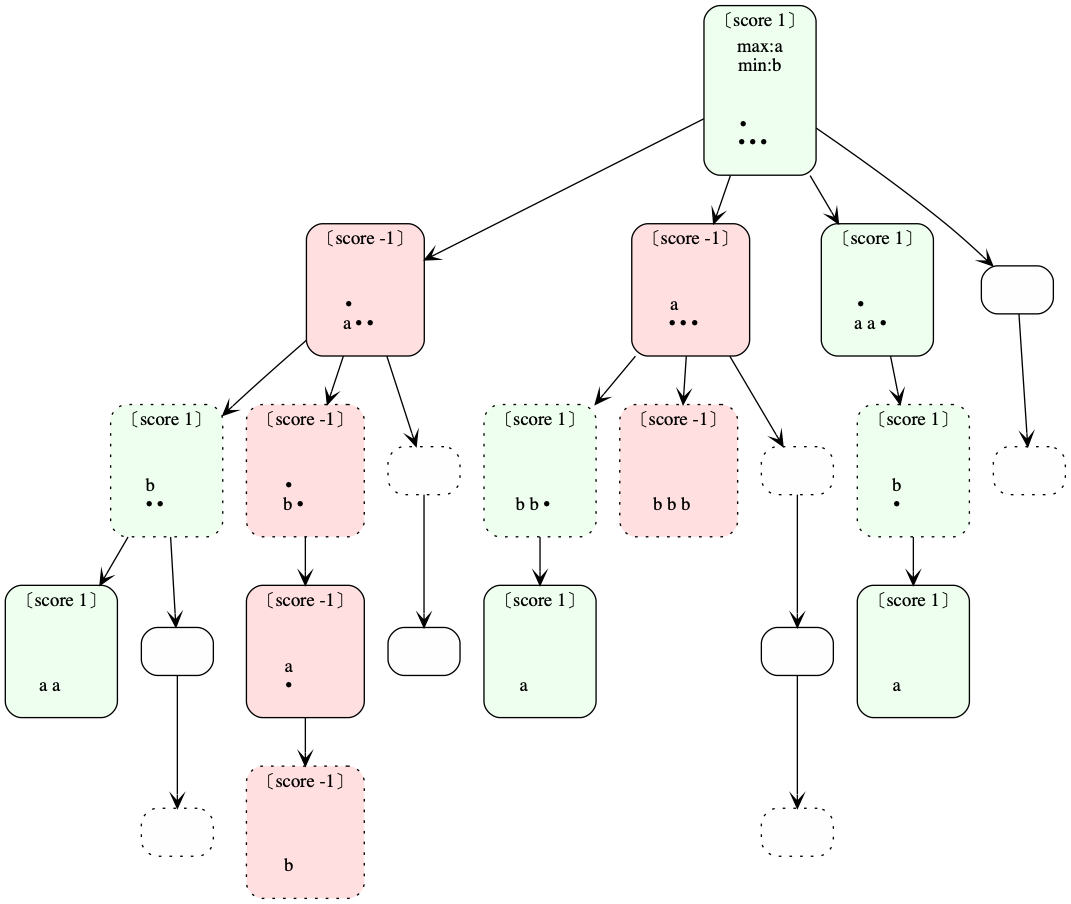
\includegraphics[width=0.9\linewidth]{tree-pruned.png}
  \caption{Tree resulting from applying the Pruned Minimax algorithm to the complete tree in Figure4. White branches are those that remain only explored by clingo but never validated.}
\end{figure}

\vspace{10px}
\textbf{Learning ASP rules}\\

During the validation process, there are some key points where we become aware of one action being better than another. This points are on lines 18, 25 and 29 of Algorithm 2 where a player should take a specific action to achieve a better reward. It is in these sections where we can generate rules that define a strategy or other type of data as explained in the next subsection. This strategy can be considered an abstract representation of the scored game tree. Within the Algorithm 2 we can easily use the current information to generate rules of the form:

\vspace{30px}

\begin{minipage}{0.90\textwidth}
  \vspace{5px}
  \begin{verbatim}
best_do(a,remove(2,2),T):-  holds(control(a),T),
                            holds(has(1,0),T), 
                            holds(has(2,2),T),
                            holds(has(3,0),T),
                            holds(has(4,0),T).
  \end{verbatim}
  \hfill
\end{minipage}
\begin{minipage}{0.05\textwidth}
  \hfill (2)
  \vspace{30px}
\end{minipage}

These rules will define under which state context, described by predicate \texttt{holds/2} is it better to perform a certain action. In this case, for the game on Nim we are stating that: In a state where player $a$ has control and only pile $2$ has $2$ counters it would be best to remove from pile $2$ both counters. 

It is important to notice that the rules in this approach will only be correct when the body defines one unique state of the game. This will imply a new requirement that must be fulfilled by the background encoding for this approach to be correct.

In order to enforce the use of these preferred actions as an strategy all we need to do is add the following rule to the strategy.

\vspace{30px}

\begin{minipage}{0.90\textwidth}
  \vspace{5px}
  \begin{verbatim}
1{does(P,A,T):best_do(P,A,T)}1:- time(T),
                                 not goal(_,_,T),
                                 {best_do(P,A,T)}>0,
                                 true(control(P)).
  \end{verbatim}
  \hfill
\end{minipage}
\begin{minipage}{0.05\textwidth}
  \hfill (3)
  \vspace{30px}
\end{minipage}


A desirable characteristic of a strategy is to be generalizable. Since the generated rules use constants, this can't be achieved. However, given a formalization allowing us to decide whether a term should be converted into a variable or not, we can substitute each some constants by variables. For this formalization we used a function $f:P,i \to Bool$ where every function name in $P$ has an associated boolean value for each attribute position $i$ indicating if it should be transformed into a variable. We will also need additional literals to ensure different variables are not substituted by the same constant during grounding. The following rule would correspond to the previous example generalized with variables using only $f(has,0)$,$f(control,0) $ and $f(best\_do,0)$ are assigned to true. 


\vspace{30px}

\begin{minipage}{0.90\textwidth}
  \vspace{5px}
  \begin{verbatim}
best_do(Va,remove(V2,1),T):-  holds(control(Va),T),
                              holds(has(V1,0),T), 
                              holds(has(V2,2),T),
                              holds(has(V3,0),T),
                              holds(has(V4,0),T),
                              V1!=V3,V1!=V2,V1!=Va,
                              V3!=V2,V3!=Va,V2!=Va.
    \end{verbatim}
  \hfill
\end{minipage}
\begin{minipage}{0.05\textwidth}
  \hfill (4)
  \vspace{30px}
\end{minipage}


With this generalize rule we can apply the strategy to any permutation over the piles and players. Further, by applying these rules during the construction of the tree we can prune more branches with the learned information. This is exemplified in figures 9 and 10. In Figure 10 we can notice how the right branch of the tree is never explored. This is because during the construction of the left branch in the bottom left corner we learned the rule mentioned above. When this rule is generalized it becomes applicable for player $b$. Since player $b$ now knows that removing two counters is better, the green section of the right branch from Figure 9 is removed leaving the only possible outcome of -1 and becoming unnecessary to be further explored by $a$.


\begin{minipage}{0.45\textwidth}
  \centering
  \vspace{10px}
  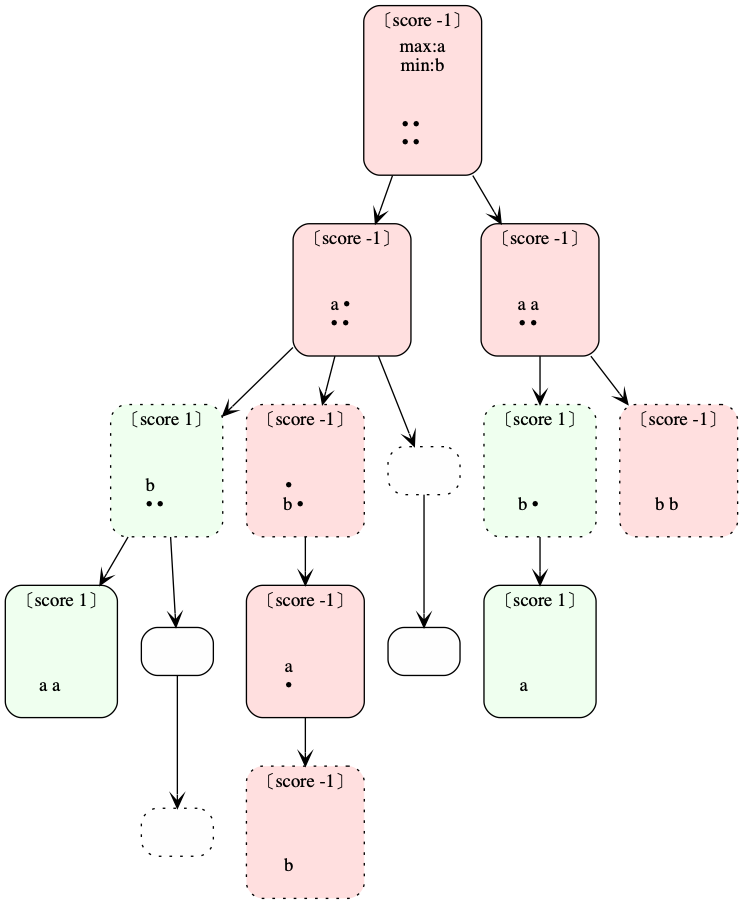
\includegraphics[height=1.3\textwidth]{tree-norules.png}
  \captionof{figure}{Pruned minimax tree without applying learned rules.}
  \vspace{15px}

\end{minipage}
\begin{minipage}{0.45\textwidth}
  \centering
  \vspace{10px}
  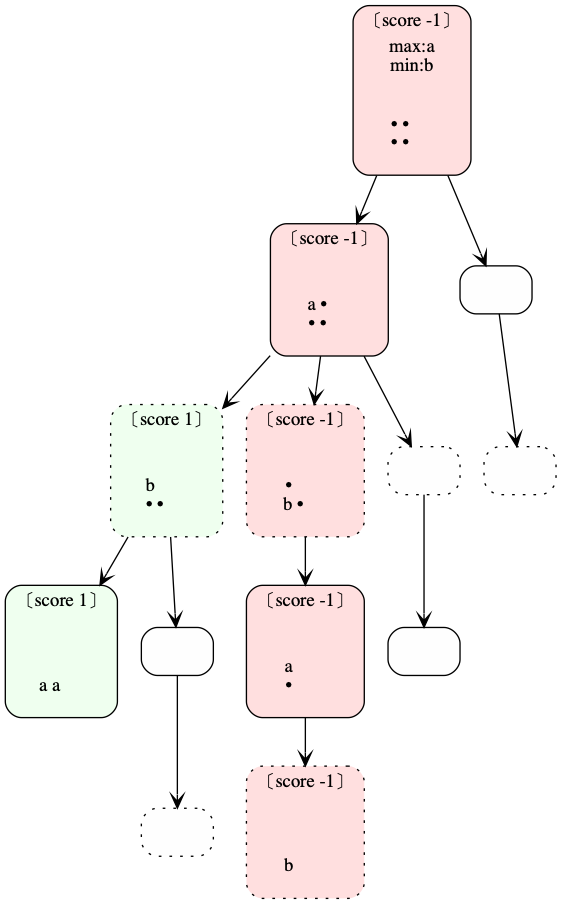
\includegraphics[height=1.3\textwidth]{tree-rules.png}
  \captionof{figure}{Pruned minimax tree applying learned rules.}
  \vspace{15px}

\end{minipage}


% \vspace{10px}
% \textbf{Generating ordered examples}\\

% The same decisive points mentioned above can also be used to generate ordered examples. 




\subsubsection{Weak Constraints from ILASP}

For this approach, our objective is to find more generalized strategies in the form of weak constraints using ILASP. Since we already have the background knowledge defined, we just need to define a set of ordered positive examples and a language bias. 

\vspace{10px}
\textbf{Generating ordered examples}\\

The decisive points mentioned in the previous section to learn rules can also be used to generate ordered examples. By running the Pruned Minimax algorithm we can construct examples with small modifications to the code. The ordered example corresponding to rule in Example 2 would be the following:

\begin{verbatim}
#pos(e0,{}, {}, {
    true(control(a)). true(has(1,0)). true(has(2,2)). 
    true(has(3,0)). true(has(3,0)). does(a,remove(2,2)). 
}).
#pos(e1,{}, {}, {
    true(control(a)). true(has(1,0)). true(has(2,2)). 
    true(has(3,0)). true(has(4,0)). does(a,remove(2,1)). 
}).

#brave_ordering(e0,e1).
\end{verbatim}

\textbf{Defining language bias}\\


Once we have the examples we only need to define a language bias. This process in most cases will require time to define how the strategy (Hypothesis) might look. The code in Figure 11 shows the language bias used for the game if TicTacToe. Line 1 to 4 define the possible atoms that might appear in the week constraint. These atoms include a cell being free, tree cells being on a line and the values for each cell. It is important to notice the use of \texttt{next/1} instead of \texttt{true/1}. Creating a strategy dependent on the next state will automatically include the effect of the action taken, thus indirectly ordering the actions. Lines 5 to 8 define the configuration for the possible weights, priorities and variables.


\begin{center}
  \begin{lstlisting}[] 
#modeo(3,next(has(var(player),var(cell))),(positive)).
#modeo(1,in_line(var(cell),var(cell),var(cell)),(positive)).
#modeo(1,next(free(var(cell))),(positive)).
#modeo(1,next(control(var(player))),(positive)).
#weight(-1).
#weight(1).
#maxp(2).
#maxv(4).
  \end{lstlisting}
  \captionof{figure}{Language bias for the game of TicTacToe}
\end{center}


For the game of Nim we wanted to find a strategy close to the mathematical one defined in \nameref{nim}. To do so, we first included in the encoding a set of facts for the binary representation of a number. Atom \texttt{binary(N,D,V)} can be read as number $N$ has the value $V\in\{1,0\}$ in position $D\in\{1,2,3\}$. Since the expected strategy is more complex and by using the existent predicates the search space is too big, we used the language bias for predicate invention. For the invention, ILASP will generate normal ASP rules in addition to the weak constraints. In the code on Figure 12, lines 5 to 7 define the invented predicates that will go in the head of the ASP rules where the body will be defined by lines 8 to 11. Lines 12 and 13 describe the possible predicates for the weak constraints.


\begin{center}
  \begin{lstlisting}[] 
#constant(pile,1).
#constant(pile,2).
#constant(pile,3).
#constant(pile,4).
#modeh(b(var(pile),var(d),var(bool)),(positive)).
#modeh(nim_sum(var(d),var(total)+var(bool),var(pile)),(positive)).
#modeh(nim_sum(var(d),0,0),(positive)).
#modeb(1,b(var(pile),var(d),var(bool)),(positive)).
#modeb(1,nim_sum(var(d),var(total),var(pile)-1),(positive)).
#modeb(1,binary(var(num),var(d),var(bool)),(positive)).
#modeb(1,next(has(var(pile),var(num))),(positive)).
#modeo(1,nim_sum(var(d),var(t),const(pile))).
#modeo(1,var(t)\2 != 0).
#weight(1).
#weight(-1).
#maxp(1).
#maxv(4).
  \end{lstlisting}
  \captionof{figure}{Language bias for the game of Nim}
\end{center}

As a final step, we will use the generated ordered examples, the language bias and the background encoding to call the ILASP framework. The call will return a hypothesis representing a strategy that will order the examples. If no Hypothesis is found the result will be UNSAT.

\newpage
\subsection{Workflow Summary}
\label{summary}
\vspace{-10pt}
\begin{figure}[H]
\centering
\begin{tikzpicture}[node distance=1cm,font=\footnotesize]
\node[vblock3, fill=green!07] (middleBig) {\vspace{-12pt} 
\begin{itemize}[leftmargin=0.5cm]
    \item[--] Background ASP/GDL rules in \texttt{background.lp}
    \item[--] Initial configuration in \texttt{*initial.lp}
    \item[--] Python \texttt{anytree} objects
    \item[--] Python-clingo API
\end{itemize}};
\node[recBlock2, below = of middleBig,fill=red!15] (prunedMinimax) {Pruned minimax};
\node[recBlock2, left = 2.0cm of prunedMinimax,fill=red!15] (basicMinimax) {Minimax};
\node[recBlock2, right = 2.0cm of prunedMinimax,fill=red!15] (combMinimax) {Pruned minimax \\ $+$ \\ Learning rules};
\node[recBlock2, below right = 1.5cm and -2cm of prunedMinimax] (orderedEgs) {Ordering examples};
\node[vblock4, below = 1cm of orderedEgs,fill=red!15] (ilasp) {ILASP framework};
\node (cross) at ($(prunedMinimax.south)+(0.0,-0.6)$) {};
\draw[<->,thick,shorten >=2pt,shorten <=2pt] (basicMinimax.north) |- (middleBig.west) {};
\draw[<->,thick,shorten >=2pt,shorten <=2pt] (prunedMinimax) -- (middleBig) {};
\draw[<->,thick,shorten >=2pt,shorten <=2pt] (combMinimax.north) |- (middleBig.east) {};
\draw[pil2] (cross.center) -| (orderedEgs.north) {};
\draw[thick] (prunedMinimax.south -| cross.north) -- (cross.center) {};
\node[recBlock2, below = 8.5cm of basicMinimax] (resBasicMinimax) {Full \\ minimax tree};
\node[recBlock2, below left = 8.5cm and -1.2cm of prunedMinimax] (resPrunedMinimax) {Pruned minimax tree};
\node[recBlock2, below right = 8.5cm and -1.2cm of prunedMinimax] (resILASP) {Weak \\constraints};
\node[recBlock2, below = 8.5cm of combMinimax] (resComb) {ASP rules};
\draw[pil2] (basicMinimax) -- (resBasicMinimax) {};
\draw[pil2] (combMinimax) -- (resComb) {};
\draw[pil2] (orderedEgs) -- (ilasp) {};
%\draw[pil] (ilasp.south) -- (resILASP.north -| ilasp.south) {};
\draw[pil2] (ilasp.south) |- ($(ilasp)!0.5!(resILASP)$) -| (resILASP.north) {};
\draw[pil2] (cross.center) -| (resPrunedMinimax) {};
\draw[pil2] (middleBig.-27) |- (ilasp.east) {};
\draw[black!60,very thick,dotted] ($(middleBig.north west)+(-3.0,0.5)$) rectangle ($(ilasp.south east)+(4.8,-0.5)$);
\draw[black!40,very thick,dotted] ($(resBasicMinimax.north west)+(-0.9,0.5)$) rectangle ($(resComb.south east)+(0.85,-0.4)$);
\node (cross2) at ($(resPrunedMinimax)!0.5!(resILASP)+(0.0,-2.0)$) {};
\draw[thick] (resBasicMinimax) |- (cross2.center) {};
\draw[thick] (resComb) |- (cross2.center) {};
\draw[thick] (resPrunedMinimax.south) -- (cross2.center -| resPrunedMinimax.south) {};
\draw[thick] (resILASP.south) -- (cross2.center -| resILASP.south) {};
\node[recBlock2] at ($(resPrunedMinimax)!0.2!(resBasicMinimax)+(0.0,-4.5)$) (build) {Build time};
\node[recBlock2] at ($(resILASP)!0.2!(resComb)+(0.0,-4.5)$) (pvp) {Player vs. random-agent};
\draw[thick,->,thick,shorten >=2pt] (cross2.center) |- (build) {};
\draw[thick,->,thick,shorten >=2pt] (cross2.center) |- (pvp) {};
\draw[black!10,very thick,dotted] ($(build.north west)+(-0.4,0.5)$) rectangle ($(pvp.south east)+(0.3,-0.4)$);
\node [left=of middleBig,yshift=2.3cm,xshift=1.9cm] {\textbf{Learning Approaches}};
\node [left=of resBasicMinimax,yshift=1.8cm,xshift=2.0cm] {\textbf{Strategies}}; 
\node [left=of build,yshift=1.85cm,xshift=2.6cm] {\textbf{Evaluation}}; 
\end{tikzpicture}
\caption{Summary of workflow/methodologies in this project separated into three different categories; namely learning approaches, strategies and evaluation}
\end{figure}

% todo: update information based on changes in previous sections
% possible: consider parallel arrows instead of superimposed
